\documentclass{article}

% If you're new to LaTeX, here's some short tutorials:
% https://www.overleaf.com/learn/latex/Learn_LaTeX_in_30_minutes
% https://en.wikibooks.org/wiki/LaTeX/Basics

% Formatting
\usepackage[utf8]{inputenc}
\usepackage[margin=1in]{geometry}
\usepackage[titletoc,title]{appendix}

% Math
% https://www.overleaf.com/learn/latex/Mathematical_expressions
% https://en.wikibooks.org/wiki/LaTeX/Mathematics
\usepackage{amsmath,amsfonts,amssymb,mathtools}

% Images
% https://www.overleaf.com/learn/latex/Inserting_Images
% https://en.wikibooks.org/wiki/LaTeX/Floats,_Figures_and_Captions
\usepackage{graphicx,float}

% Tables
% https://www.overleaf.com/learn/latex/Tables
% https://en.wikibooks.org/wiki/LaTeX/Tables

% Algorithms
% https://www.overleaf.com/learn/latex/algorithms
% https://en.wikibooks.org/wiki/LaTeX/Algorithms
\usepackage[ruled,vlined]{algorithm2e}
\usepackage{algorithmic}

% Code syntax highlighting
% https://www.overleaf.com/learn/latex/Code_Highlighting_with_minted
\usepackage{listings}
%\usepackage{minted}
%\usemintedstyle{borland}

\usepackage{hyperref}
\usepackage{subcaption}
\usepackage{bm}

% References
% https://www.overleaf.com/learn/latex/Bibliography_management_in_LaTeX
% https://en.wikibooks.org/wiki/LaTeX/Bibliography_Management
%\usepackage{biblatex}
%\addbibresource{references.bib}

% Title content
\title{AMATH 582 Project: DMD of a weak turbulence}
\author{Daniel W. Crews}
\date{March 10, 2021}

\begin{document}

\maketitle

% Abstract
\begin{abstract}
  This project analyzes simulation of a classic problem in collisionless plasma turbulence called the bump-on-tail instability using dynamic mode decomposition (DMD), where spatiotemporally-correlated modes of varying complex frequencies are determined. The bump-on-tail instability describes collisionless relaxation of a superthermal electron beam towards thermodynamic equilibrium. Relaxation occurs through Cherenkov emission of longitudinal plasma waves, leading to a broad distribution of wave energy and a dynamic, weakly turbulent distribution on averaged scales. The problem is solved by evolving the electron distribution function's Boltzmann equation in phase space, setting up its natural observables as the fluid moments projected onto the position and velocity axes. This work pretends not to know about the full phase space information and considers DMD analysis of the observables only, as well as the DMD modes of the Wigner function of spatial wavepackets arising through instability.

%  looks at a simple example of the DMD by solving the problem of video background separation. This is accomplished by subtracting the lowest frequency modes from a video clip, with the wrinkle of negative pixel values dealt with in video-dependent ways. Generally negative values can simply be subtracted out. Yet in a video of a skiier, the snow is much brighter than the skiier so subtracting out negative values removes the skiier too. For this clip, the negative pixels are flipped to their absolute values. %he DMD has many other significant uses such as in linear control theory.
  %Measurements generically include superfluous components (from the perspective of an analyst at least). An old, efficient, and quite spectacular method to extract particular dynamics within a dataset is called principal component analysis (PCA). Basically, PCA is an eigendecomposition of the covariance matrix. This report utilizes PCA to analyze simple harmonic motion recorded on separate video cameras, assigning different oscillatory components to particular modal coordinates rather their motional ones. %rather than dispersed between various different ones. % Spectral analysis consists of far more than determination of the Fourier coefficients of a time series. This numerical experiment explores the spatial distribution of a signal's frequency spectrum (or spectrogram) through the pratical examples of classic shredding moments in music history (here, Guns and Roses and Pink Floyd). To compute the spectrograms a short-time (masked) Fourier transform is used, and in particular this report explores its filtering using the Wigner distribution function of the time series. Here the Wigner function is computed as an $\mathcal{O}(N^2)$ operation in terms of the Fourier coefficients.
    %Signal processing is used ubiquitously in science and engineering. This simple numerical experiment explores an important aspect of signal analysis, namely statistical averaging of a spectral time series to eliminate noise and thereby identify center frequencies. Here the time series consists of a spatial wavefield which is denoised via Gaussian filtering about the identified frequency to determine a trajectory. While the technique explored in this report is quite elementary compared to more sophisticated signal processing approaches, it conveys the essential elements of, for example, a radar or sonar tracking system. %In this case such a trajectory is determined from a noisy waveform in a time series of three spatial dimensions. 
\end{abstract}

% Introduction and Overview
\section{Introduction and Overview}
When an experimenter observes a plasma's distribution function they determine an average $\langle f\rangle$ over scales and realizations owing to their instrumentation's resolution. Now consider a numerical experiment wherein one solves microscopic, deterministic equations on some domain with specified initial and boundary conditions. The numerical experimenter obtains a facsimile of the physical experimenter's observations by considering distributions averaged over appropriate scales (such as the domain), effecting a ``computational coarse-graining'' of time or space scales. In this way the spatially-averaged distribution $\langle f\rangle_x$ and fluid moments $\langle v^nf\rangle_v$ may be considered observable quantities of a simulation of the Vlasov-Poisson systems. Figure \ref{projection} shows a schematic overview of the phase space projections as observables associated with phase flow.

\begin{figure}[hb!]
  \centering
  \includegraphics[width=0.5\textwidth]{projection}
  \caption{Phase flow is associated natural observable quantities, the mean velocity distribution $\langle f\rangle_v$ and the fluid moments $\langle v^0f\rangle\equiv n(x)$, $\langle vf\rangle$, $\langle v^2f\rangle$, etc. Reduced models for collisionless plasma processes attempt to describe dynamics of the projected variables without detailed knowledge of the phase space structure.}\label{projection}
\end{figure}

% The first section of this report briefly summarizes the SVD theory and that of the linear classifiers, before proceeding into the results of analysis in the second section. Here the various classification methods are compared to one another, in particular on difficult-to-distinguish digit pairs. However, here it's found that the SVM method sorts these with good accuracy. While this analysis utilized the entire training and test dataset and hence had a deterministic outcome, in practical application of these methods cross-validation (repeated classification with a randomly sampled training dataset) is needed to demonstrate robustness.
%Here four expriments are analyzed of videos taken from three perspectives of a mass oscillating at the end of a string. The four experiments consisted of simple one-dimensional harmonic motion in gravity from the string tension, then introduction of an additional swinging pendulum motion, and thirdly also rotation of the oscillating mass. Finally data was collected with camera shake in order to introduce measurement noise. The measurements are composed of multiple relatively independent simultaneously occuring oscillations to demonstrate the mathemagical properties of the principal component analysis (PCA) method, which separates oscillatory modes by an eigendecomposition (thus, diagonalization) of the data covariance matrix.

%The purpose of this work is to visualize some of the most famous shredding in rock and roll history (Pink Floyd and Guns and Roses (GNR)) by construction of a spectrogram. Section \ref{theory} outlines the theory of the combined Gabor-Wigner distribution used for the spectrogram, followed by a section detailing implementation of the algorithm. Results are presented for the opening guitar riff in GNR, bass line in Floyd, and a stab at the Floyd guitar solo. The attached appendices describing elements of Wigner distributions are hoped not to count towards the overall page limit and included merely for completeness. The report itself is kept concise.

% This report describes an algorithm used to denoise the signal via a statistical method and to identify the submarine's trajectory. It begins with a brief theoretical overview of the methods used, and proceeds to a discussion of the details of the code used to implement the methods. There is then a discussion of results identifying the three-dimensional trajectory, along with a suggested search area for a submarine-tracking aircraft and the likely frequency of the submarine. The report is kept brief without sacrificing clarity.

% Theoretical Background
\section{Theoretical Background}\label{theory}
\subsection{Quasilinear weak turbulence theory}
The first approximation to velocity-space diffusion in electrostatic turbulence is known as the quasilinear approximation. This basically says that the first approximation to the evolution of the observable distribution $\langle f\rangle_L$ is a heat equation. The reader can skip it. The theory is a reduction from the Vlasov-Poisson equations,
\begin{align}
  \partial_tf &+ v\partial_xf - \frac{q}{m}\partial_x\varphi\partial_vf = 0,\label{vlasov}\\
  \partial_x^2\varphi(x) &= \frac{q}{\epsilon_0}(n_e - n_i),\label{poisson}\\
  n_e &\equiv \int_{-\infty}^\infty f(v)dv, \quad n_i \equiv \langle n_e\rangle
\end{align}
describing collective collisionless behavior as a phase flow conserving probability. Generally one gives a Gaussian initial condition with some perturbation. The average distribution function evolves far from Gaussian during evolution of an instability. If the average wave energy is weak, one can apply quasilinear theory. Here the distribution function is expanded into average and fluctuating parts,
\begin{align}
  f(x,v,t) &= f_0(X, v, t) + f_1(x, v, t)\\
  f_0(X,v,t) &= \langle f\rangle_L,\quad\quad f_1(x,v,t) = f-\langle f\rangle_L,\quad \langle f_1\rangle_L = 0.
\end{align}
In a manner completely analogous to Reynolds averaging, one expands the Vlasov equation, spatially averages, and subtracts the mean to obtain the fluctuating equation,
\begin{align}
  \frac{\partial f}{\partial t} + v\frac{\partial f}{\partial x} + \frac{q}{m}E\frac{\partial f}{\partial v} = 0&\implies \frac{\partial f_0}{\partial t} + \frac{q}{m}\Big\langle\frac{\partial f_1}{\partial v}E_1\Big\rangle = 0\\
  \text{using the averaged equation } &\implies \frac{\partial f_1}{\partial t} + v\frac{\partial f_1}{\partial x} + \frac{q}{m}\frac{\partial f_0}{\partial v}E_1 = 0
\end{align}
where in the second equation the variation of the fluctuating force
\begin{equation}
  \frac{q}{m}\Big(\frac{\partial f_1}{\partial v}E_1 - \Big\langle\frac{\partial f_1}{\partial v}E_1\Big\rangle\Big)\label{dropped}
\end{equation}
is considered to be higher-order and dropped for closure, making the evolution of the fluctuation $f_1$ a linear equation whose inhomogeneous part is the flux due to acceleration of the \textit{bulk} distribution \cite{thorne}. Some remarks are in order on the equation for the background,
\begin{equation}
  \frac{\partial f_0}{\partial t} = -\frac{q}{m}\frac{\partial}{\partial v}\langle f_1E_1\rangle_L \label{background_eqn}
\end{equation}
which states that the driver of the observable distribution $f_0 = \langle f\rangle$ is due to the difference in flux $\langle f_1E_1\rangle$, or \textit{the unnormalized field-particle correlation coefficient} \cite{vankampen}. The quasilinear closure, dropping Eqn. \ref{dropped}, amounts to supposing that the correlation has zero variance. Under the assumption of linearity of the fluctuation, Fourier transform the equation for $f_1$,
\begin{equation}
  \widetilde{f}_1 = -\frac{q}{m}\frac{i}{\omega - kv}\frac{\partial f_0}{\partial v}\widetilde{E}_1
\end{equation}
and consider in the continuous spectrum limit $L\to\infty$ the average fluctuating force as
\begin{align}
  \frac{\partial }{\partial v}\Big\langle f_1E_1\Big\rangle &= \frac{\partial}{\partial v}\Big(\frac{1}{L}\int_0^Lf_1Edx\Big) \approx \frac{\partial}{\partial v}\Big(\frac{1}{L}\int_{-\infty}^\infty f_1Edx\Big)\\
  &= \frac{\partial}{\partial v}\Big(\int_{-\infty}^\infty\frac{dk}{2\pi}\frac{\widetilde{E}_1^*\widetilde{f}_1}{L}\Big)
\end{align}
where in the last equality Parseval's equality has been used to convert the integrand to spectral variables \cite{thorne}. Then substitution of $\widetilde{f}_1$ yields
\begin{equation}
  \frac{\partial }{\partial v}\Big\langle f_1E_1\Big\rangle = -\frac{q}{m}\frac{\partial}{\partial v}\Big(\int_{-\infty}^\infty\frac{dk}{2\pi}\frac{\widetilde{E}_1^*\widetilde{E}_1}{L}\frac{i}{\omega - kv}\frac{\partial f_0}{\partial v}\Big)\label{mean_fluc_accel}
\end{equation}
where for causality here $\omega_i > 0$ is taken to have positive imaginary part (a more careful analysis using the Laplace transform arrives at Landau's form for all such resonant integrals). Define the spectral energy density as $\mathcal{E}(k) = \frac{\epsilon_0\widetilde{E}_1^*\widetilde{E}_1}{2\pi L}$. This form of the correlation closes the equation for the average distribution $f_0$ provided that $\mathcal{E}(k)$ is known. By noting the plasma frequency $\omega_p^2 = \frac{nq^2}{\epsilon_0m}$, define the diffusion coefficient
\begin{equation}
  D(v) = \frac{\omega_p^2}{nm}\int_{-\infty}^\infty\frac{i}{\omega - kv}\mathcal{E}(k)dk\label{ql_diffusivity}
\end{equation}
with which one obtains the \textit{quasilinear diffusion equation} for evolution of $f_0$,
\begin{equation}
  \frac{\partial f_0}{\partial t} = \frac{\partial}{\partial v}\Big(D(v)\frac{\partial f_0}{\partial v}\Big)\label{ql_equation}.
\end{equation}
The spectrum $\mathcal{E}(k)$ and dispersion relation $\omega(k) = \omega_r(k) + i\omega_i(k)$ remain to be determined. The simplest equation for evolution of the spectrum follows from trigonometry \textit{assuming no modal interactions} (which take the form of a ``collision'' term) and slow modulations,
\begin{equation}
  \mathcal{E}\sim E^2\sim e^{2i\omega t}\implies \frac{d\mathcal{E}}{dt} = 2\omega_i\mathcal{E}\label{spect}
\end{equation}
and for the dispersion relation, one examines the roots of the linear dielectric function,
\begin{equation}
  \epsilon(\omega, k) = 1 + \frac{\omega_{pe}^2}{m_ek}\int_{\mathcal{L}}\frac{1}{\omega - kv}\frac{\partial g}{\partial v}dv = 0\label{dielectric}
\end{equation}
where $g = f_e + \sum_s\frac{m_e}{m_s}f_s$ is the unified distribution function which sums over different plasma species. Equations \ref{ql_diffusivity} - \ref{dielectric} form a closed, diffusive system to describe the background distribution. However, when an instability saturates the energy is typically larger than the threshold for this purely diffusive approximation to hold true, and other fluctuations are observed. The DMD analysis attempts to see this effect.

\subsection{Dynamic mode decomposition}
In this class, a data matrix was often decomposed into its proper modes using the SVD operation. These frames, such as handwriting examples, were not time-dependent. In simulation of Eqns. \ref{vlasov} and \ref{poisson}, each timestep is separated from its neighbors by a time difference $\Delta t$. If the data is collected into an array $X\in\mathbb{R}^{n\times m}$ of dimension (phase space$\times$time), and a second array $X'$ is formed one difference $\Delta t$ into the future, then the two may be supposed to be related by a Koopman evolution operator,
\begin{equation}
  X' = AX
\end{equation}
where $A$ is taken to solve the problem in the least-squares Moore-Penrose pseudoinverse $Y^+$ sense \cite{kutz}. However, this makes $A = X'X^+$ a (pixels$\times$pixels) operator. Generally speaking this matrix $A$ will be too large to perform an eigenvalue decomposition on directly with any efficiency. On the other hand, dynamic mode decomposition tackles this problem by projecting into a low-rank truncation of $X$ obtained via SVD,
\begin{equation}
  X_r = U_r\Sigma_rV_r^\dagger
\end{equation}
with $r$ the truncation order. Therefore the Koopman operator $A$ may be represented in this subspace,
\begin{equation}
  \widetilde{A} \equiv U_r^\dagger A_rU_r = U^\dagger X'V_r\Sigma_r^{-1}
\end{equation}
with $\widetilde{A}\in\mathbb{C}^{r\times r}$. Having identified an approximate $A$, a more tractable eigendecomposition is performed
\begin{equation}
  \widetilde{A}W = W\Lambda.\label{eigs}
\end{equation}
The orthogonal modes of the low-dimensional evolution operator are then lifted to the full-rank space by
\begin{equation}
  \Phi \equiv X'V_r\Sigma_r^{-1}W
\end{equation}
and the fundamental frequencies computed via $\Omega \equiv \log(\Lambda)/\Delta t$. By this method the DMD has been accomplished according to the approximate continuous-time reconstruction
\begin{equation}
  \widetilde{X}(t) = \Phi\exp(\Omega t)b
\end{equation}
where $b$ is the vector of initial conditions obtained via $b = \Phi^+X(0)$. This reconstruction is approximate in the sense that high mode dynamics have been disregarded \cite{kutz_dmd}.

% \subsection{Background subtraction method}\label{background}
% The above is the standard DMD method. In this work, a slight variation is used to perform the background subtraction. By examination of the eigenvalue spectrum $\Lambda$ of the low-dimensional operator of Eqn. \ref{eigs}, the lowest frequency modes $\Lambda_L$ (usually just one or two) are extracted and its reduced eigenvector $W_L$ used to construct the low-frequency DMD operator $\Phi_L$ \cite{kutz_dmd}. The method then proceeds as normal. A slight variation on the method presented in Ref. \cite{kutz_dmd} is used, wherein the best-fit background $b(t)$ is identified for each time increment by calculating $b(t_i) = X(t_i)\Phi^+$ rather than exponentially evolving the frequencies. This was found to work better, but they are perhaps equivalent and the author may simply have had a bug.

% Algorithm Implementation and Development
\section{Full simulation results}\label{section}
One way of ensuring the smallness of the terms in Eqn. \ref{dropped} is that the excited waves are i) small amplitude, e.g. from a weak instability, and ii) are part of a wide family of excited wavenumbers for a continuous range of resonant phase velocities. A problem which fits the conditions of a weakly interacting broad spectrum is called a weak wave turbulence. According to criteria developed in Thorne and Blandford (Ref. \cite{thorne}), such a distribution is given by a hot distribution drifting through a main Maxwellian's tail,
\begin{equation}
  f_0(v) = \frac{1}{(1+\chi)\sqrt{2\pi}}\Bigg[\frac{1}{v_{t0}}\exp\Bigg(-\frac{v^2}{2v_{t0}^2}\Bigg) + \frac{\chi}{v_{t1}}\exp\Bigg(-\frac{(v-v_b)^2}{2v_{t1}^2}\Bigg)\Bigg]
\end{equation}
with parameters chosen in the weak turbulence regime with i) bump fraction $\chi = 0.05$, ii) bump spread $v_{t1} = \chi^{1/3}v_b$, and iii) beam velocity $v_b = 5v_{t0}$. The distribution and the growth rates corresponding to Eqn. \ref{dielectric} are shown in Fig. \ref{ic_ql}. Such a problem is referred to as the bump-on-tail (BOT) instability. The instability can be thought of as the means by which a nonequilibrium distribution releases free energy and relaxes closer to thermal equilibrium through Cherenkov emission mediated by collective interactions.

\begin{figure}[hb!]
  \centering
  \includegraphics[width=0.5\textwidth]{chap2/initial_condition}\includegraphics[width=0.42\textwidth]{chap2/initial_growth_newer}
  \caption{Initial electron distribution $\langle f\rangle_L$ and instability growth rate $\omega_i/\omega_p$ for the bump-on-tail problem. A broad spectrum of Langmuir waves is excited between $k\lambda_D \sim 0.23-0.45$.}\label{ic_ql}
\end{figure}
Figures \ref{sol_ql_full} and \ref{vp_tail} show the results of the quasilinear approximation and from direct numerical numerical simulation of the instability, respectively, as well as the Koopman operator's complex frequencies $\omega = \log(\Lambda)/\Delta t$ upon DMD of the observable in the direct simulation. Most modes grow with the instability. 
\begin{figure}[ht]
  \centering
  \includegraphics[width=0.42\textwidth]{full_quad_jan24/full_dist}\includegraphics[width=0.55\textwidth]{full_quad_jan24/dist_zoom}
  %\includegraphics[width=0.45\textwidth]{chap2/ql_right/whole_dist_doubleD}\includegraphics[width=0.45\textwidth]{chap2/ql_right/tail_flat_doubleD}
  \caption{Evolution of bulk distribution $f_0(v)$ (left) and tail flattening (right) in quasilinear approximation of bump-on-tail instability. Approach to the steady-state is necessarily asymptotic.}\label{sol_ql_full}
\end{figure}
\begin{figure}[h]
  \centering
  \includegraphics[width=0.5\textwidth]{high_res/tail}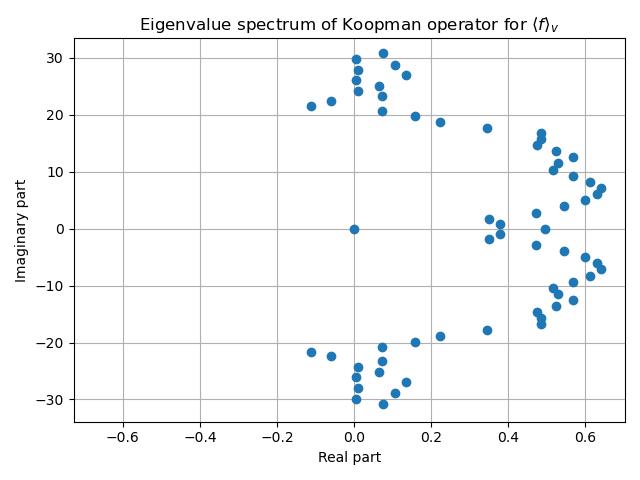
\includegraphics[width=0.4255\textwidth]{avgf/pdf_dmd_freqs_zoom}%\includegraphics[width=0.4\textwidth]{tavg_saturated}
  \caption{(Left:) Tail flattening of the background $\langle f\rangle_L$ in the electron bump-on-tail instability in a Vlasov-Poisson simulation on $L=1000\lambda_D$. Observable diffusion proceeds according to quasilinear theory. Important differences are a smaller change in energy of the bulk electrons than in the QL approximation, and a faster rate of smoothing the high-velocity edge. (Right): DMD Koopman complex frequencies of $\langle f\rangle_L$. All parts grow away from the initial condition, which sits squarely at the zero mode occupying a lot of energy.}\label{vp_tail}
\end{figure}
\begin{figure}[h]
  \centering
  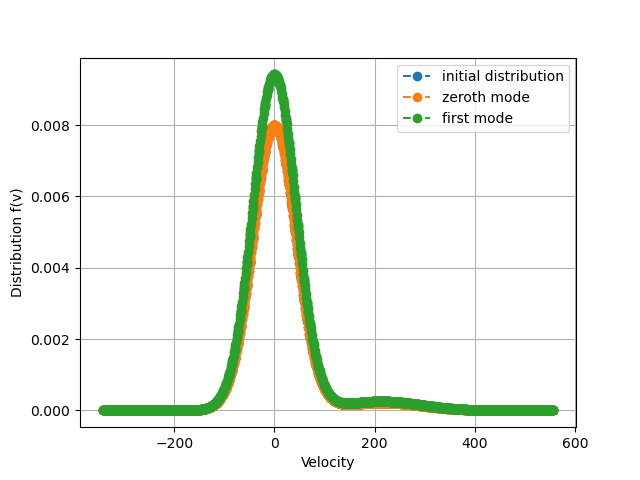
\includegraphics[width=0.45\textwidth]{avgf/avg_f_koopman_modes}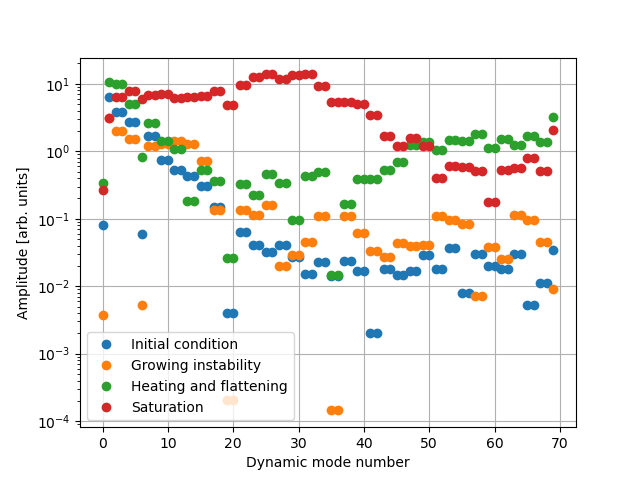
\includegraphics[width=0.45\textwidth]{avgf/avg_f_modal_amplitudes}
  \caption{(Left): First DMD modes of $\langle f\rangle$, with the zeroth mode totally overlapping the initial distribution. The larger first mode captures a small change in the background distribution arising due to a small heating of the background distribution due to the instability. (Right): Four snapshots in time of the DMD modal spectrum of $\langle f\rangle$. At saturation, many modes are needed to describe the tail flattening!}
\end{figure}

As well, Fig. \ref{density} shows the wavefield of Langmuir waves arising from the instability up to saturation. These wavepackets generically obey a Klein-Gordon type dispersion relation $\omega^2 \sim \omega_p^2 + \langle v^2\rangle k^2$, which is approximately nonlinear Schr\"{o}dinger dynamics for these long wavelengths, yet with a growing term.
\begin{figure}[t]
  \centering
  \includegraphics[width=0.35\textwidth]{high_res/density}\includegraphics[width=0.5\textwidth]{lang_dopp}
  \caption{The observable density $n(x)$ at saturation (left) contains a field of wavepackets propagating to the right with the Langmuir group velocity. This translational invariance was removed (right) by a phase shift.}\label{density}
\end{figure}
\begin{figure}
  \centering
  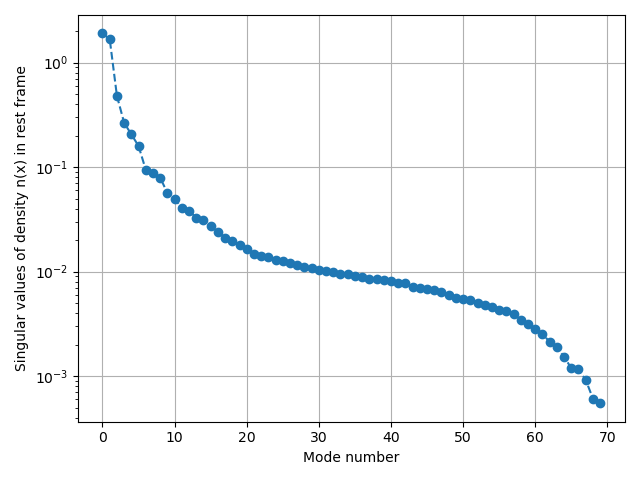
\includegraphics[width=0.45\textwidth]{density/density_svs_groupframe}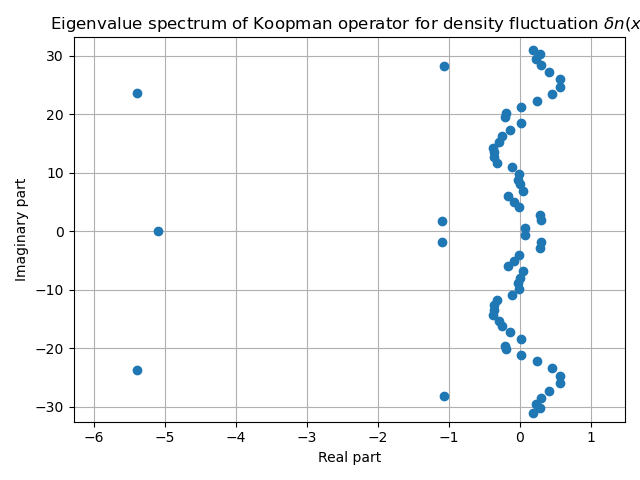
\includegraphics[width=0.45\textwidth]{density/density_dmd_freqs_zoom}
  \caption{(Left): Singular values of the wavefield after removing translational invariance, which previously was not a sparse spectrum. Instead it is dominated by just two modes. (Right): Complex frequencies of the Koopman operator in DMD of the time-dependent wavefield.}\label{density_dmd}
\end{figure}
\begin{figure}
  \centering
  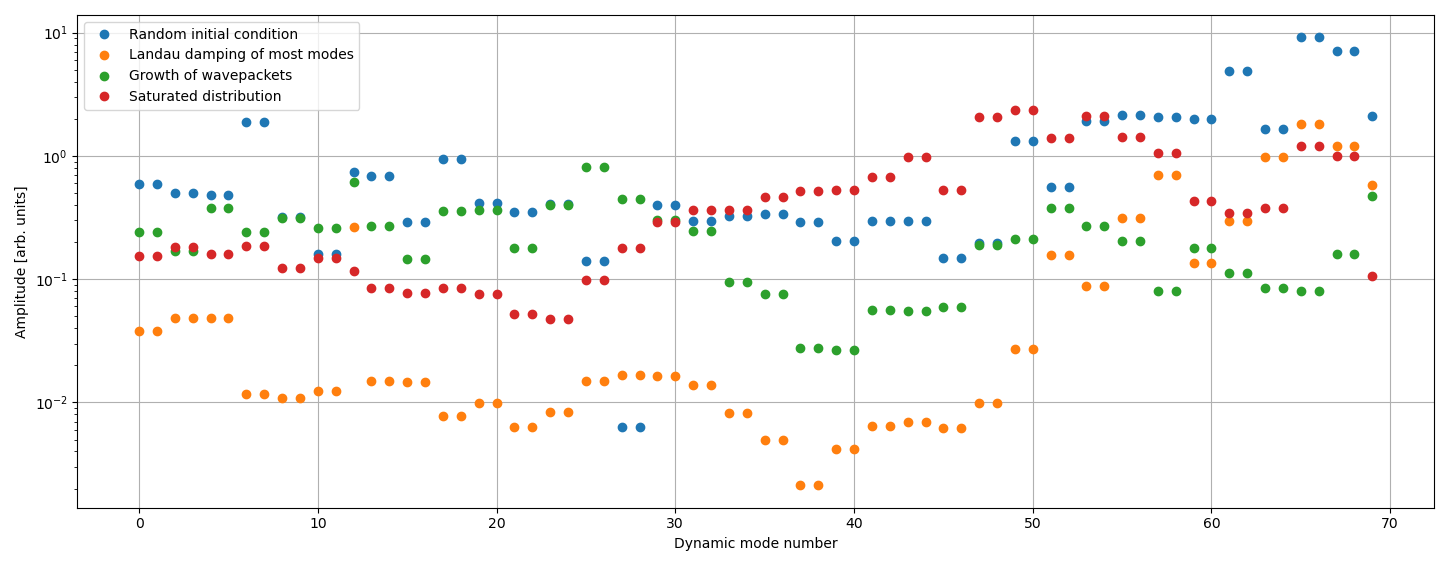
\includegraphics[width=\textwidth]{density/density_dmd_modes}
  \caption{Four time snapshots of the DMD modal spectrum of $\langle f\rangle$, organized by absolute value of the DMD frequency. Initialized by a random wavefield, waves are first damped by collisionless processes, before growing due to the instability. The final spectrum is dominated by the modes which grew, occupying the higher modes seen here.}
\end{figure}

Further, Fig. \ref{tapestry} shows the complex phase space dynamics occuring during evolution of the instability.
\begin{figure}[b]
  \centering
  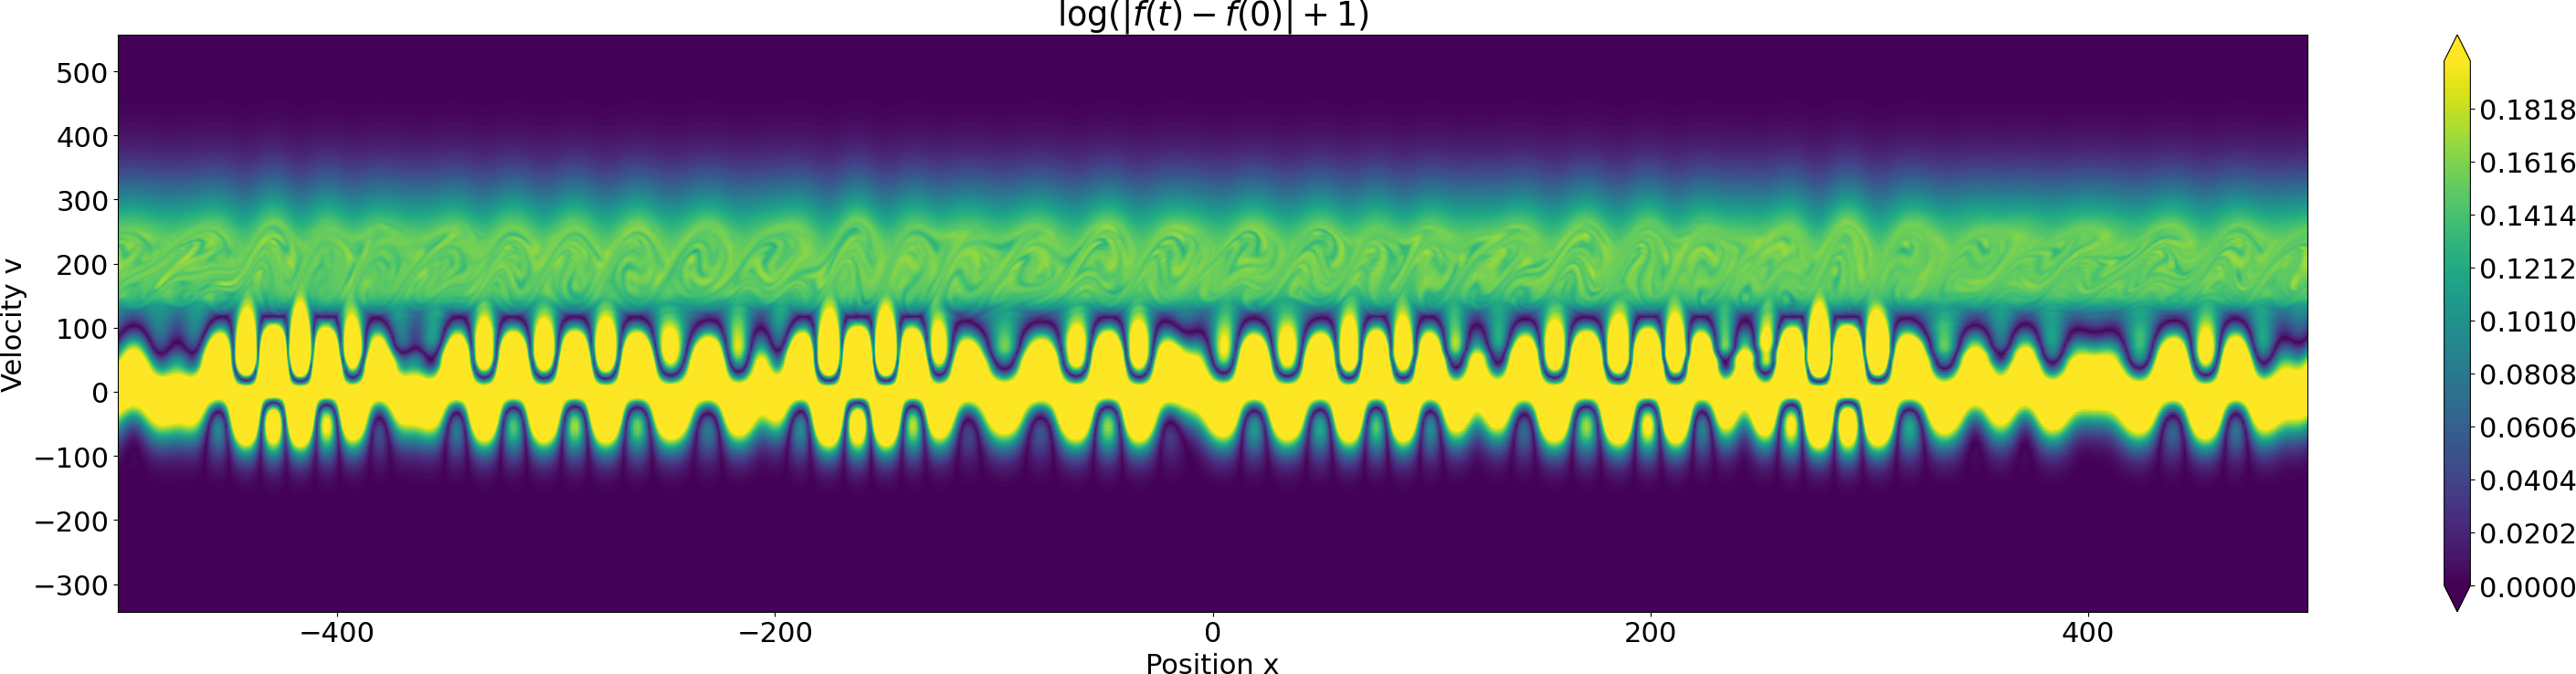
\includegraphics[width=\textwidth]{tapestry}
  \caption{Logarithmic plot of the difference from the initial condition at saturation of the bump-on-tail instability. Highly-correlated wave structures are present, as well as a more chaotic region of particle trapping around the wave phase velocities.}\label{tapestry}
\end{figure}


% Each video consists of a number of frames at sixty frames-per-second. These are loaded in, converted to grayscale, and then analyzed by the DMD algorithm of Section \ref{theory}. For each video the low-rank truncation of $X_r$ used to construct $\widetilde{A}$ was chosen to be 100 modes. The resulting eigenvalue spectrum of of $\widetilde{A}$ is shown in Fig. \ref{eigs_pics_mc} and \ref{eigs_pics_sd} for the race cars and skiier respectively. It was found that four race car modes and five skiier ones were sufficient for background reconstruction. Experimentation on the precise number of low-frequency modes was found not to be significant provided that there were enough of them, \textit{but} not too many.

% \begin{figure}[b!]
%   \centering
%   \includegraphics[width=0.45\textwidth]{montecarlo_dmd_spectrum}\quad\quad\quad\includegraphics[width=0.45\textwidth]{montecarlo_low_spectrum}
%   \caption{Spectrum of the low-rank approximate race car Koopman operator $\widetilde{A}$ using an $r=100$ truncation. Evidently the the low-frequency activity is clustered around a cloud of modes. The four lowest modes were found to provide a good low-frequency reconstruction according to the method of Section \ref{background}.}\label{eigs_pics_mc}
% \end{figure}

% \begin{figure}[t!]
%   \centering
%   \includegraphics[width=0.45\textwidth]{skidrop_dmd_spectrum}\quad\quad\quad\includegraphics[width=0.45\textwidth]{skidrop_low_freq_spectrum}
%   \caption{Eigenvalues of the skiier video operator approximated with one hundred modes. Here, the sparse background is observed to occupy mostly one mode, with a far sparser low-frequency spectrum than the race car video. The five smallest modes are used to account for slight variations and background wobble.}\label{eigs_pics_sd}
% \end{figure}


% \begin{figure}[hb!]
%   \centering
%   \includegraphics[width=0.45\textwidth]{skiier_color}\quad\quad\quad\includegraphics[width=0.455\textwidth]{skiier}
%   \caption{The skiier against a beautiful mountain scene (left) and with the background subtracted (right).}\label{skiiers}
% \end{figure}

% \begin{figure}[ht!]
%   \centering
%   \includegraphics[width=0.45\textwidth]{racecars3}\quad\quad\quad\includegraphics[width=0.455\textwidth]{racecars3_nbg}
%   \caption{Race cars in a fancy European city (left) and without their background (right).}\label{montecarlo}
% \end{figure}

% \begin{figure}[hb!]
%   \centering
%   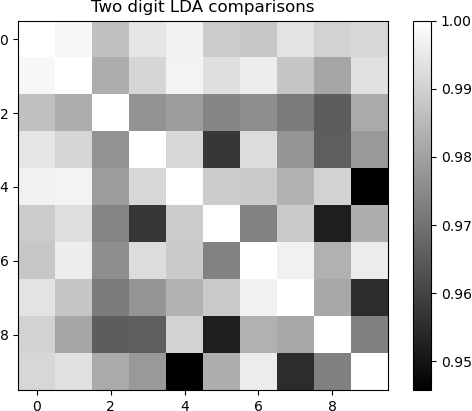
\includegraphics[width=0.4\textwidth]{2dgt_error_lda_50modes}\quad\quad\quad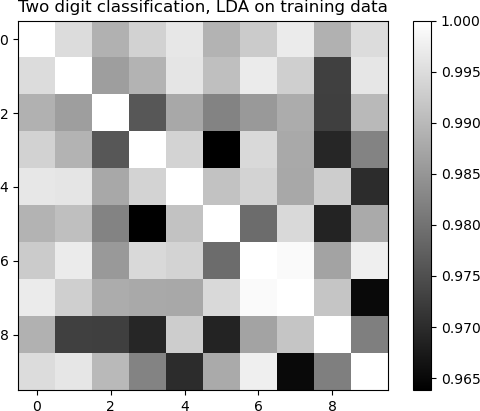
\includegraphics[width=0.4\textwidth]{ontrainingdata/lda_allmodes}
%   \caption{Classification score of LDA method on digit pairs. (Left:) scores of the test data using 50-mode reduced training data. While all scores are $>94$\%, 2 has a poor trend and certain pairings are not good.\\(Right:) Classifier score on its own training data without dimension reduction, showing inherent LDA error.}\label{lda}
% \end{figure}

% \begin{figure}[ht!]
%   \centering
%   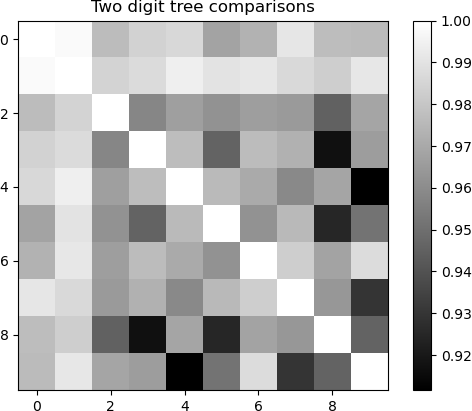
\includegraphics[width=0.4\textwidth]{2dgt_tree_50modes}\quad\quad\quad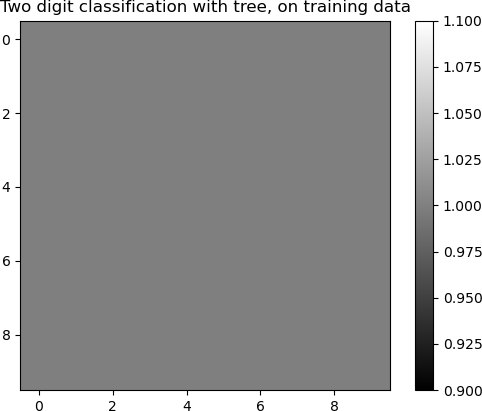
\includegraphics[width=0.4\textwidth]{ontrainingdata/tree_training}
%   \caption{(Left:) Two-digit classification results using the decision tree method. Interestingly, larger errors are observed compared to the LDA, but the digit 2 consistently performs better. Errors on the difficult-to-distinguish pairs of the LDA are exacerbated by the decision tree. (Right:) The tree, at least with default settings, predicts its own training data exactly (so the colorbar was autoset). This indicates overfitting.}\label{tree}
% \end{figure}

% Further, predicting the original training data reveals the very same error pattern, though at a lower rate of incidence. This demonstrates an inherent error in the LDA method due to outliers, even though it operates on a minimized Rayleigh quotient. Now Fig. \ref{tree} demonstrates results with the decision tree method. The main takeaway from these results is that errors on difficult-to-distinguish data are made even worse by the decision tree compared to the LDA, but it predicts its own training data very well.

% Next, the support vector machine was explored with results in Fig. \ref{svm}. The SVM was observed to be calculated faster than the decision tree \textit{and} to have accurate results to within almost 1\%! However, it has a small rate of error in predicting its own training data. As before, the SVM was trained on a 50-mode reduced dimension eigenprojected dataset. Comparison of Figs. \ref{lda}, \ref{tree}, and \ref{svm} shows that all three methods distinguish 0 and 1 very well, and all have the most difficulty with 4 and 9. However, the SVM classifier predicts with great accuracy and beats the others by several percentage points.

% It must be stressed that this analysis is done deterministically on a single set of training and test data. Generally speaking these methods are to be cross-validated by randomly sampling a subset of the training data and doing a statistical analysis of the resulting scores for different training set sizes. The author played around with this a bit while doing the assignment but did not include these results for brevity. The general trend was that scores were lower when using a smaller training set, but the SVM still did the best.

% \begin{figure}[hb!]
%   \centering
%   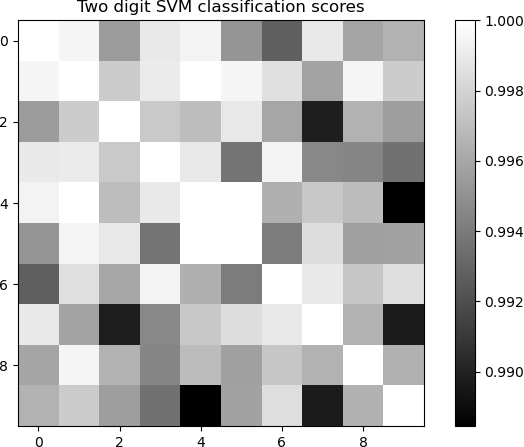
\includegraphics[width=0.4\textwidth]{2dgt_svm_50modes}\quad\quad\quad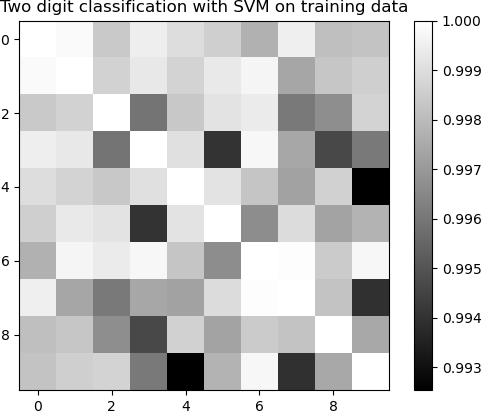
\includegraphics[width=0.4\textwidth]{ontrainingdata/svm_training}
%   \caption{Two-digit classification results with the SVM method. The support vector technique is seen to be the best of the three methods overall, and intriguingly has almost perfect discernment between digits 4 and 5. It stumbles most on 4 and 9, however perhaps even a human would on these digits when handwritten.}\label{svm}
% \end{figure}

% \begin{figure}[ht!]
%   \centering
%   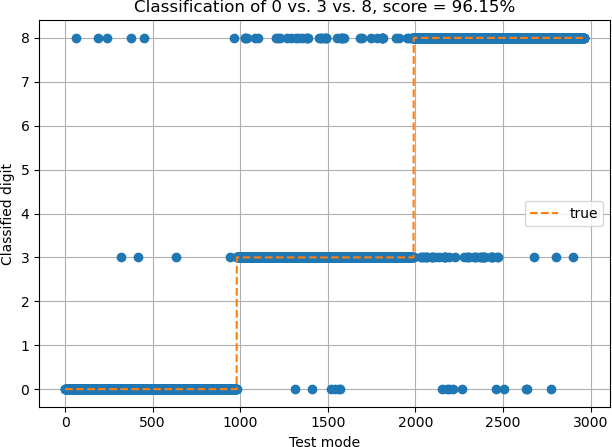
\includegraphics[width=0.315\textwidth]{lda3/3digit_lda_038}\quad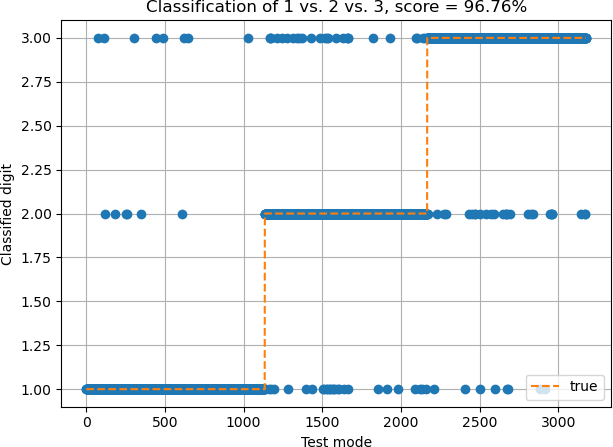
\includegraphics[width=0.315\textwidth]{lda3/3digit_lda_123}\quad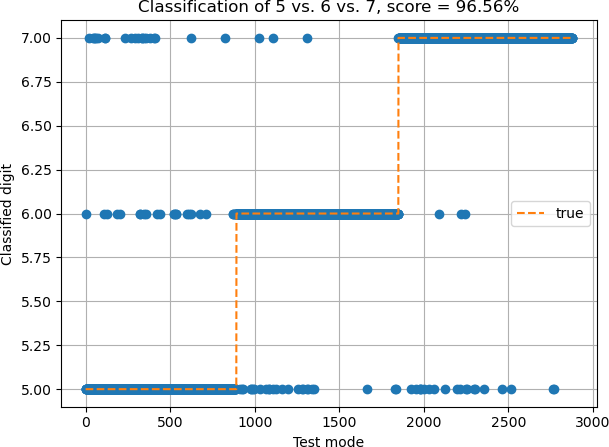
\includegraphics[width=0.315\textwidth]{lda3/3digit_lda_567}
%   \caption{Simultaneous classification of three digits using LDA on the sets of digits 038, 123, and 567. Generally good classification in line with the ``worst'' results of the two-digit LDA is observed, here $> 96$\%.}\label{threedigit}
% \end{figure}

% \subsection{Three-digit classification}
% As an initial exploration of further capabilities, Fig. \ref{threedigit} shows LDA applied to categorize three digits simultaneously. Good results are seen in these cases, with general trends in line with the results of the two-digit LDA in Fig. \ref{lda}. However, one would expect that simultaneous classification of all nine digits would run into issues due to the general mixing of eigenvalues for the difficult pairs such as 9 and 4, contaminating performance of the entire classification scheme. Three digits was generally seen to work well though.

% \begin{figure}[h]
%   \centering
%   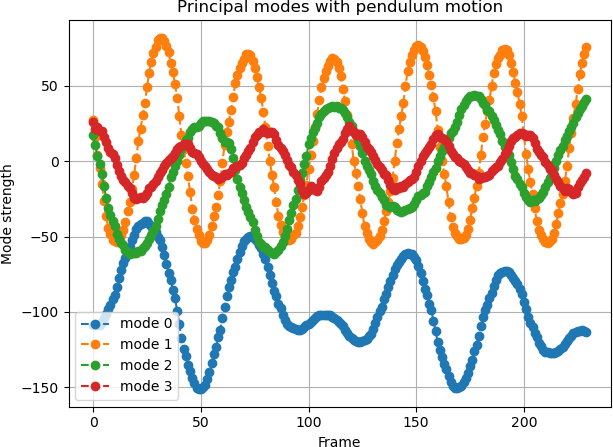
\includegraphics[width=0.45\textwidth]{pca_pend2}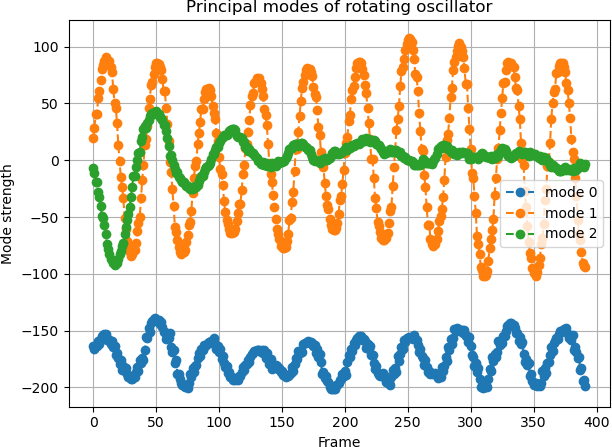
\includegraphics[width=0.45\textwidth]{pca_rotate2}
%   \caption{Projected modes of bucket coordinates for cases of SHM superimposed on pendulum motion (left) and bucket rotation (right). In comparison to the baseline case (Fig. \ref{sns}) clearly ``mode 1'' still describes the bucket SHM as their frequencies match. The pendulum motion appears as a lower-frequency oscillation apparently in ``mode 2''. However, the occurence of both oscillations appears to leave a modulated trace (superposition?) in mode 0, in curious correlation with the Wigner function experiments of the last homework. The rotating oscillator case shows a damped rotation tendency in ``mode 2,'' matching the video here.}\label{pr}
% \end{figure}

% \begin{figure}[hb!]
%   \centering
%   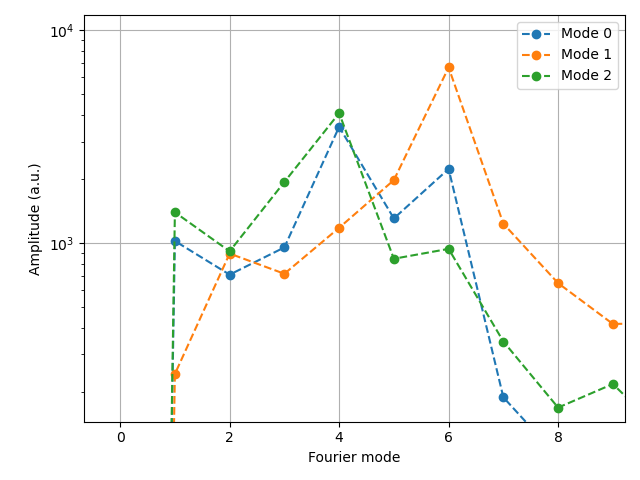
\includegraphics[width=0.5\textwidth]{pendulum_fft3}
%   \caption{First few Fourier components from FFT of the pendulum case, showing the frequencies in the ``mode 0'' waveform to be the SHM and pendulum frequencies 4 and 6, and perhaps interference in mode 5.}\label{pend_fft}
% \end{figure}

% \begin{table}[b]
%   \centering
%   \begin{tabular}{|l|l|l|l|l|l|l|l|l|}
%     \hline
%     Time {[}hr{]}   & 0-3.5 & 3.5-7.0 & 7.0-10.5 & 10.5-14.0 & 14.0-17.5 & 17.5-21.0 & 21.0-24.5 & All-time average \\ \hline
%     $\langle k_x\rangle_T$ {[}1/L{]} & 0.814 & 0.661   & 0.784    & 0.760     & 0.810     & 0.728     & 0.802     & 0.766            \\ \hline
%     $\langle k_y\rangle_T$ {[}1/L{]} & 0.271 & 0.292   & 0.331    & 0.240     & 0.341     & 0.267     & 0.271     & 0.288            \\ \hline
%     $\langle k_z\rangle_T$ {[}1/L{]} & -1.00 & -1.03   & -1.09    & -1.06     & -1.13     & -1.07     & -1.1125   & -1.07            \\ \hline
%   \end{tabular}
%   \caption{Observed center frequencies of data following spectral averaging over time intervals of $3.5$ hours, with seven samples per interval, then used as the filter frequencies $k_0$ in the Gaussian filter. The arbitrary spatial unit is given as $L$, not to be confused with domain length. The all-time average is given as well.}\label{frequencies}
% \end{table}

% Note that in Table \ref{frequencies} negative wavenumbers are used as the given spatial data is complex, meaning that the reality condition is not satisfied, instead $\hat{f}(-k) = \hat{f}^*(k)$ in this dataset. The absolute value is reported as ``the frequency'' of the submarine, however. This identifies the submarine's spectral signature as $\bm{k} \approx \{0.766 \pm 0.05, 0.288 \pm 0.03, 1.07 \pm 0.04 \}$ {[}1/L{]} by mean and standard deviation of the window averages of Table \ref{frequencies}, where L is an arbitrary space unit corresponding to that of the provided data, \textit{not} the domain length. The width of the space or frequency ``submarine Gaussian'' was not measured for ease of analysis.

% Having computed the center frequencies, the spectrum was filtered and the trajectory determined according to the schematic Steps 4 and 5. The resulting 3D trajectory and top-down position given in Figs. \ref{traj:3d}, \ref{traj:2d} respectively. This suggests the submarine is currently located around $\bm{x}\sim(-5, 6.5)$ in $(x,y)$.

% \begin{figure}[hb]
%   \centering
%   \begin{subfigure}{0.42\textwidth}
%     \centering
%     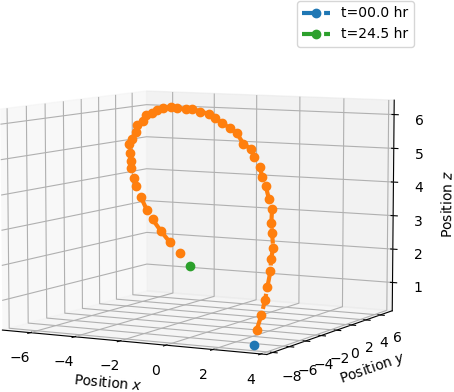
\includegraphics[width=0.99\linewidth]{pics/3d_traj}
%     \caption{Three-dimensional trajectory of submarine, showing a rise and dive maneuver.}\label{traj:3d}
%   \end{subfigure}
%   \begin{subfigure}{0.42\textwidth}
%     \centering
%     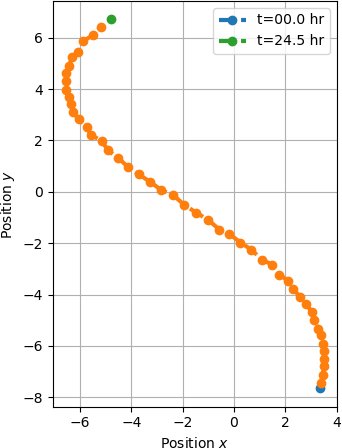
\includegraphics[width=0.6\linewidth]{pics/2d_traj}
%     \caption{Top-down view of predicted trajectory. Ideal search area for submarine-tracking aircraft is around $\bm{x} \sim (-5, 6.5)$ and continuing north-east.}\label{traj:2d}
%   \end{subfigure}
%   \caption{Identified submarine trajectory sampled 49 times in a 24.5 hour period, in 3D and 2D projections.}
% \end{figure}

% Summary and Conclusions
\section{Summary and Conclusions}
This numerical experiment considered a DMD analysis of the data obtained by direct numerical simulation of a classic plasma instability. Of note was that the eigenvalues of the Koopman operator all grew, indicative of an instability. The resulting spectra were generally not easy to interpret, although the author was surprised by how well the DMD pulled out the background of the observables. More work remains to be done to study the use of DMD to analyze these types of problems.
% \begin{figure}[b!]
%   \centering
%   \includegraphics[width=0.425\textwidth]{racecars_av}
%   \caption{The absolute value of the sparse reconstruction $|X_S(t)|$ gave better image quality than Fig. \ref{montecarlo2} yet with more artifacts such as the street appearing on top of the car, seen here on the left side of the first car.}\label{montecarlo2}
% \end{figure}

% % References
\bibliographystyle{unsrt}
\bibliography{references}

% \begin{figure}[t!]
%   \centering
%   \includegraphics[width=0.65\textwidth]{montecarlo_background}\quad\includegraphics[width=0.3\textwidth]{skidrop_background2}
%   \caption{Background reconstructions of race cars (left) and skiier (right) using the low-frequency modes.}\label{backgrounds}
% \end{figure}

% % Appendices
\begin{appendices}

% \newpage
% % MATLAB Functions
% \section{Python Functions}\label{functions}
% The following list compiles important Python functions used in implementation:
% \begin{itemize}
% \item The commands \texttt{np.linalg.svd(X)} and \texttt{np.linalg.eig(X)} are used for big linear algebra operations,
% \item The \texttt{av} package was used to read in the \texttt{.mp4} video clips,
% \item The sequence \texttt{np.argsort(np.abs(freqs))} sorts the eigenvalues by their absolute value.
% \end{itemize}

% % MATLAB Codes
%\section{Python Implementation}\label{implementation}
% A separate analysis script was used for each dataset and the files are quite similar. Only pendulum is shown for brevity (see Github page for other files).
% % Wigner function file \texttt{fourier.py}:
% \lstinputlisting{wpendulum.py}
% \vspace{5cm}
%Main implementation file \texttt{hw5.py}:
%\lstinputlisting{hw5.py}
% \begin{listing}[h]
% \inputminted{matlab}{example.m}
% \caption{Example code from external file.}
% \label{listing:examplecode}
% \end{listing}

\end{appendices}

\end{document}